\documentclass{article}


\usepackage{../template/template}

\usepackage[utf8]{inputenc} % allow utf-8 input
\usepackage[T1]{fontenc}    % use 8-bit T1 fonts
\usepackage{hyperref}       % hyperlinks
\usepackage{url}            % simple URL typesetting
\usepackage{booktabs}       % professional-quality tables
\usepackage{amsfonts}       % blackboard math symbols
\usepackage{nicefrac}       % compact symbols for 1/2, etc.
\usepackage{microtype}      % microtypography
% \usepackage{lipsum} 產生隨機文章,沒用!

% 設定 CJK 中文字體

% 設定 highlighting 套件

\providecommand{\tightlist}{%
  \setlength{\itemsep}{0pt}\setlength{\parskip}{0pt}}

\title{一種基於 xxx 的模擬改良方法}

\author{
      陳鍾誠 \\
    國立金門大學資訊工程系 \\
    \texttt{ccc@nqu.edu.tw}
    \and
      Mitchell John \\
    NASA \\
    \texttt{MitchellJohn@gmail.com}
    \and
  }

\begin{document}
\maketitle

\begin{abstract}
  簡短介紹這篇論文的主要貢獻與使用方法等等,例如:本文提出一種基於 xxx
  的方法,可以在 ooo 的條件下進行 xxx 的模擬 \ldots..
\end{abstract}

% keywords can be removed
\keywords{
   xxx \and  ooo \and 
}

\hypertarget{ux7c21ux4ecb}{%
\section{簡介}\label{ux7c21ux4ecb}}

在此描述您的作品或研究動機、背景 \ldots{}

\hypertarget{ux6587ux737bux56deux9867}{%
\section{文獻回顧}\label{ux6587ux737bux56deux9867}}

介紹一下目前其他人的研究成果並具體舉出文獻,例如 Kour and Saabne (2014),
Hadash et al. (2018) 等等, \ldots.

接著介紹你的方法有何優勢等等 \ldots{}

\hypertarget{ux7814ux7a76ux65b9ux6cd5}{%
\section{研究方法}\label{ux7814ux7a76ux65b9ux6cd5}}

描述您的方法或技術,您也可以使用數學式將您的方法更清楚地描述出來!

\[
L(X;\theta)=P(X|\theta)=\sum_z P(X,z|\theta) \\
\arg\max_{\theta_{t+1}} \frac{\sum_i P(x_i|\theta)}{n}\\
\]

\hypertarget{ux5be6ux9a57ux7d50ux679c}{%
\section{實驗結果}\label{ux5be6ux9a57ux7d50ux679c}}

您可以用圖表展現實驗結果 \ldots.

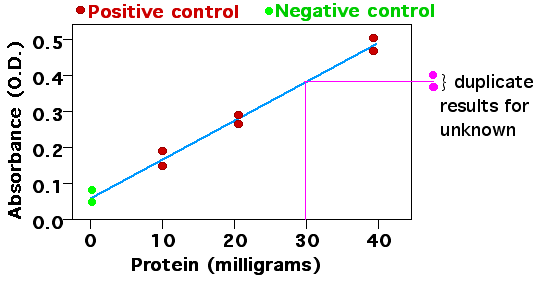
\includegraphics{img/curve.png}

也可以用表格進行分析

\begin{longtable}[]{@{}lll@{}}
\toprule
實驗 & 正確率 & 說明\tabularnewline
\midrule
\endhead
方法 1 & 82.34\% & 用 xxx 資料測試\tabularnewline
方法 2 & 85.51\% & 用 ooo 資料測試\tabularnewline
方法 3 & 94.33\% & 用 xxx 資料測試\tabularnewline
\bottomrule
\end{longtable}

\hypertarget{ux7d50ux8a9e}{%
\section{結語}\label{ux7d50ux8a9e}}

說明你的方法之優點與限制,還有甚麼需要改進的未來展望等等 \ldots{}

\hypertarget{ux53c3ux8003ux6587ux737b}{%
\section*{參考文獻}\label{ux53c3ux8003ux6587ux737b}}
\addcontentsline{toc}{section}{參考文獻}

\hypertarget{refs}{}
\leavevmode\hypertarget{ref-hadash2018estimate}{}%
Hadash, Guy, Einat Kermany, Boaz Carmeli, Ofer Lavi, George Kour, and
Alon Jacovi. 2018. ``Estimate and Replace: A Novel Approach to
Integrating Deep Neural Networks with Existing Applications.''
\emph{arXiv Preprint arXiv:1804.09028}.

\leavevmode\hypertarget{ref-kour2014fast}{}%
Kour, George, and Raid Saabne. 2014. ``Fast Classification of
Handwritten on-Line Arabic Characters.'' In \emph{Soft Computing and
Pattern Recognition (Socpar), 2014 6th International Conference of},
312--18. IEEE.


\end{document}
